\chapter{Sistemas de reducción abstractos}

En este capítulo, definiremos que entendemos como un sistema de
reducción abstracto, y a partir de este, daremos la definición de
orden, que sera imprescindible para capítulos posteriores. También
veremos en qué consiste la inducción bien fundada, el orden
lexicográfico y un poco de teoría de multiconjuntos. Estas dos últimas
incluirán una implementación en Haskell que se puede encontrar en
\texttt{Orden.hs}


\section{Equivalencia y reducción}

El objetivo principal de esta sección es definir toda la estructura de
los sistemas de reducción abstractos.

\begin{defi} 
  Un \textbf{sistema de reducción abstracto} es un par $(A, \rightarrow)$ donde
  la reducción $\rightarrow$, es una relación en el conjunto $A$; es decir,
  $\rightarrow \subseteq A \times A$.
\end{defi}

Para simplificar la notación, si $(a,b) \in \rightarrow$, escribiremos
$a\rightarrow b$.  Un sistema de reducción abstracto se puede entender
como un grafo dirigido. Por ejemplo,

\begin{figure}[h]
          \centering
          \begin{tikzpicture}
          \begin{scope}[execute at begin node=$, execute at end node=$]
          \node (v1) at (0,0) {a};
          \node (v2) at (3,0) {b};
          \node (v3) at (6,1) {c};
          \node (v4) at (6,-1) {d};
          \end{scope}
          
          \draw [-latex](v2) (v1) edge  node [auto] {} (v2);
          \draw [-latex](v3) (v2) edge  node [auto] {} (v3);
          \draw [-latex](v4) (v2) edge  node [auto] {} (v4);
          \draw [-latex](v1) (v2) edge [bend right] node [auto] {} (v1);
          \end{tikzpicture}
\end{figure}

\begin{defi} 
  Diremos que $b$ es una \textbf{reducción} de $a$ si
  $a\rightarrow a_0 \rightarrow a_1\rightarrow \dots\rightarrow b$.
\end{defi}

En el ejemplo anterior, $c$ es una reducción de $a$. Pero $d$ no es
una reducción de $c$

\begin{defi} 
  Diremos que $a$ y $b$ son \textbf{equivalentes}, y lo denotaremos por
  $a \xleftrightarrow{*} b$, si $b$ es una reducción de $a$ y $a$ es una
  reducción de $b$.
\end{defi}

En el ejemplo, $a$ y $b$ son equivalentes.
También trabajaremos con el concepto de composición.

\begin{defi} 
  Dadas dos relaciones $R \subseteq A\times B$, y $S \times B \times C$,
  definimos su \textbf{composición} como
  \[R \circ S := 
    \left\lbrace (x,z)\in A \times C | \exists y \in B. (x,y) \in R \wedge (y,z) \in S \right\rbrace   \]
\end{defi}

A partir de una reducción $\rightarrow$ se pueden calcular diferentes clausuras,

\begin{defi} 
  A partir de la definición de reducción, consideraremos las siguientes nociones, \\
  $\begin{array}{llll}
     \xrightarrow{0}         & := & \left\lbrace (x,x) | x \in A \right\rbrace   & $\textbf{Identidad}$  \\ 
     \xrightarrow{i+1}       & := & \xrightarrow{i}$ ó $ \rightarrow & \textbf{(i+1)}$\textbf{-plegado,} $  \pmb{i\geq 0} \\ 
     \xrightarrow{+}         & := & \cup_{i>0} \xrightarrow{i} & $\textbf{Clausura transitiva}$ \\ 
     \xrightarrow{*}         & := & \xrightarrow{+} \cup \xrightarrow{0} & $\textbf{Clausura transitiva reflexiva}$ \\ 
     \xrightarrow{=}         & := & \rightarrow \cup \xrightarrow{0} & $\textbf{Clausura reflexiva}$ \\ 
     \xrightarrow{-1} & := & \left\lbrace (y,x) | x\rightarrow y \right\rbrace  & $\textbf{Inversa}$ \\ 
     \leftarrow      & := & \xrightarrow{-1} & $\textbf{Inversa}$ \\ 
     \leftrightarrow         & := & \rightarrow \bigcup \leftarrow & $\textbf{Clausura simétrica}$ \\ 
     \xleftrightarrow{+}     & := & \left( \leftrightarrow \right)^{+} & $\textbf{Clausura transitiva simetrica}$ \\ 
     \xleftrightarrow{*}     & := & \left( \leftrightarrow \right)^{*} & $\textbf{Clausura reflexiva transitiva simetrica}$
   \end{array} 
   $
\end{defi}

\begin{ejem}
  A partir de la reducción:
  \begin{figure}[h]
          \centering
          \begin{tikzpicture}
          \begin{scope}[execute at begin node=$, execute at end node=$]
          \node (v1) at (0,0) {a};
          \node (v2) at (3,0) {b};
          \node (v3) at (6,1) {c};
          \node (v4) at (6,-1) {d};
          \node (v5) at (9,-2) {e};
          \end{scope}
          
          \draw [-latex](v2) (v1) edge  node [auto] {} (v2);
          \draw [-latex](v3) (v2) edge  node [auto] {} (v3);
          \draw [-latex](v4) (v2) edge  node [auto] {} (v4);
          \draw [-latex](v5) (v4) edge  node [auto] {} (v5);
          
  
          \end{tikzpicture}
  \end{figure}    
  Las relaciones según la definición anterior son,
  \begin{figure}[h]
          \centering
          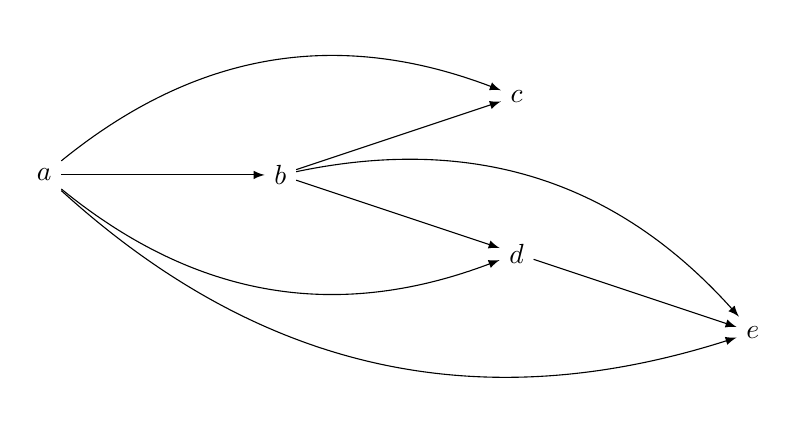
\begin{tikzpicture}
          \begin{scope}[execute at begin node=$, execute at end node=$]
          \node (v1) at (0,0) {a};
          \node (v2) at (3,0) {b};
          \node (v3) at (6,1) {c};
          \node (v4) at (6,-1) {d};
          \node (v5) at (9,-2) {e};
          \end{scope}
          
          \draw [-latex](v2) (v1) edge  node [auto] {} (v2);
          \draw [-latex](v3) (v2) edge  node [auto] {} (v3);
          \draw [-latex](v4) (v2) edge  node [auto] {} (v4);
          \draw [-latex](v5) (v4) edge  node [auto] {} (v5);
          \draw [-latex](v4) (v1) edge [bend right] node [auto] {} (v4);
          \draw [-latex](v5) (v1) edge [bend right] node [auto] {} (v5);
          \draw [-latex](v3) (v1) edge [bend left] node [auto] {} (v3);
          \draw [-latex](v5) (v2) edge [bend left] node [auto] {} (v5);
          
          
          \end{tikzpicture}
          \caption{$\xrightarrow{+}$}
  \end{figure}            
  \begin{figure}[h]
          \centering
          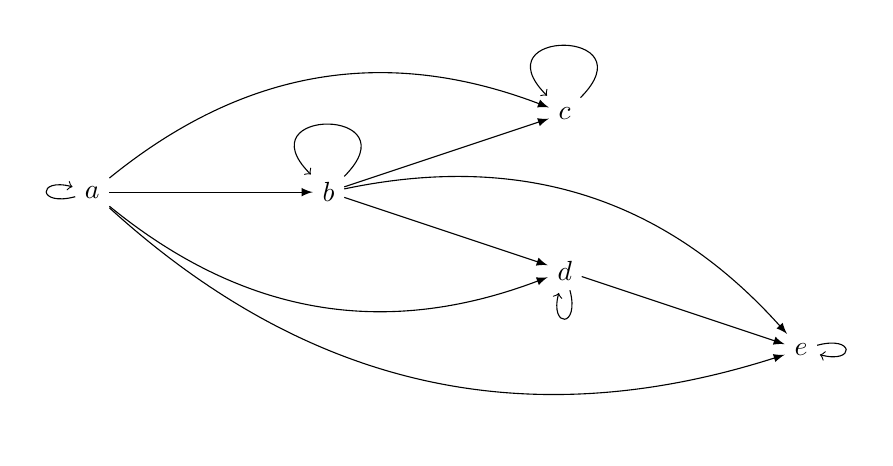
\begin{tikzpicture}
          \begin{scope}[execute at begin node=$, execute at end node=$]
          \node (v1) at (0,0) {a};
          \node (v2) at (3,0) {b};
          \node (v3) at (6,1) {c};
          \node (v4) at (6,-1) {d};
          \node (v5) at (9,-2) {e};
          \end{scope}
          
          \draw [-latex](v2) (v1) edge  node [auto] {} (v2);
          \draw [-latex](v3) (v2) edge  node [auto] {} (v3);
          \draw [-latex](v4) (v2) edge  node [auto] {} (v4);
          \draw [-latex](v5) (v4) edge  node [auto] {} (v5);
          \draw [-latex](v4) (v1) edge [bend right] node [auto] {} (v4);
          \draw [-latex](v5) (v1) edge [bend right] node [auto] {} (v5);
          \draw [-latex](v3) (v1) edge [bend left] node [auto] {} (v3);
          \draw [-latex](v5) (v2) edge [bend left] node [auto] {} (v5);
          \draw [-latex](v2) (v1) edge [loop left] node [auto] {} (v2);
          \draw [-latex](v3) (v2) edge [loop] node [auto] {} (v3);
          \draw [-latex](v5) (v4) edge [loop below] node [auto] {} (v5);
          \draw [-latex](v5) (v3) edge [loop] node [auto] {} (v5);
          \draw [-latex](v5) (v5) edge [loop right] node [auto] {} (v5);
          
          \end{tikzpicture}
          \caption{$\xrightarrow{*}$}
  \end{figure}            
\end{ejem}

A continuación, veremos una serie de definiciones que serán
imprescindibles a la hora de estudiar los sistemas de reescritura.

\begin{defi} 
  Diremos que $P$ es la \textbf{clausura} de $R$ si $P$ es el menor conjunto
  con la propiedad $P$ que contiene a $R$.
\end{defi}

\begin{defi} 
  Diremos que $x$ es \textbf{reducible} si existe un $y$ tal que
  $x \rightarrow y$.
\end{defi}

\begin{defi} 
  Diremos que $x$ esta en su \textbf{forma normal} si $x$ no es reducible.
\end{defi}

%\begin{defi} 
%  Diremos que $\pmb{y}$ \textbf{es la forma normal de} $\pmb{x}$ si
%  $x \xrightarrow{*} y$, donde $y$ es una forma normal. Si $x$ tiene una única
%  forma normal, lo denotaremos por $x \downarrow$.
%\end{defi}

%\begin{defi} 
%  Diremos que $y$ es un \textbf{sucesor directo} de $x$ si $x \rightarrow y$.
%\end{defi}

\begin{defi} 
  Diremos que $y$ es un \textbf{sucesor} de $x$ si $x \xrightarrow{+} y$
\end{defi}      

\begin{defi} 
  Diremos que $x$ e $y$ son \textbf{confluentes} si hay algún $z$ tal que
  $x\xrightarrow{*}z \xleftarrow{*} y$. Lo denotaremos por $x \downarrow y$.
\end{defi}      

%Ejemplos 2.1.2 1)

\begin{defi} 
  Llamaremos a una reducción $\rightarrow$, \\
  $       
  \begin{array}{ll}
    $\textbf{Church-Rosser}$        & $si $ x \xleftrightarrow{*} y \Leftrightarrow x \downarrow y \\ 
    $\textbf{confluente}$   & $si $ y_1 \xleftarrow{*} x \xrightarrow{*} y_2 \Rightarrow y_1 \downarrow y_2\\ 
    $\textbf{semi-confluente}$      & $si $ y_1 \leftarrow x \xrightarrow{*} y_2 \Rightarrow y_1 \downarrow y_2\\ 
    $\textbf{terminante}$   & $si no hay una cadena infinita $ a_0 \rightarrow a_1 \rightarrow \dots \\ 
    $\textbf{normalizado}$  & $si cada elemento tiene forma normal$\\ 
    $\textbf{convergente}$  & $si es confluente y terminante$
  \end{array}     
  $
\end{defi}

La línea discontinua en los siguientes diagramas representa la
existencia de una reducción. Por ejemplo, en Church Rosser nos indica que si $ x \xleftrightarrow{*} y$, entonces $\exists z$ tal que $x \xleftrightarrow{*} z $, e $y \xleftrightarrow{*} z$

%Church Rosser
\begin{figure}[h]
  \centering
  \begin{tikzpicture}
          \node (v1) at (0,3) {x};
          \node (v2) at (3,3) {y};
          \node (v3) at (1.5,0.8) {z};
          
          \draw [latex-latex](v2) (v1) edge  node [auto] {*} (v2);
          \draw [latex-latex, dash pattern=on 2pt off 3pt on 4pt off 4pt](v3)  edge  node [auto] {*} (v1);
          \draw [latex-latex, dash pattern=on 2pt off 3pt on 4pt off 4pt](v2)  edge  node[auto] {*} (v3);
  \end{tikzpicture}
  \caption{Church Rosser}
\end{figure}

%Confluente
\begin{figure}[h]
  \centering
  \begin{tikzpicture}
    \begin{scope}[execute at begin node=$, execute at end node=$]
      \node (v3) at (0,0) {y_2};
      \node (v1) at (0,3) {x};
      \node (v4) at (3,0) {z};
      \node (v2) at (3,3) {y_1};
      \end{scope}
      
      \draw [-latex](v2) (v1) edge  node [auto] {*} (v2);
      \draw [-latex](v3) (v1) edge  node [left] {*} (v3);
      \draw [-latex, dash pattern=on 2pt off 3pt on 4pt off 4pt](v3)  edge  node [below] {*} (v4);
      \draw [-latex, dash pattern=on 2pt off 3pt on 4pt off 4pt](v2)  edge  node[auto] {*} (v4);
  \end{tikzpicture}
  \caption{Confluente}
\end{figure}

%Semi-confluente
\begin{figure}[h]
  \centering
  \begin{tikzpicture}
    \begin{scope}[execute at begin node=$, execute at end node=$]
      \node (v3) at (0,0) {y_2};
      \node (v1) at (0,3) {x};
      \node (v4) at (3,0) {z};
      \node (v2) at (3,3) {y_1};
      \end{scope}
      
      \draw [-latex](v2) (v1) edge  node [auto] {} (v2);
      \draw [-latex](v3) (v1) edge  node [left] {*} (v3);
      \draw [-latex, dash pattern=on 2pt off 3pt on 4pt off 4pt](v3)  edge  node [below] {*} (v4);
      \draw [-latex, dash pattern=on 2pt off 3pt on 4pt off 4pt](v2)  edge  node[auto] {*} (v4);
  \end{tikzpicture}
  \caption{Semi-confluente}
\end{figure}

\section{Resultados básicos}

A partir de las anteriores definiciones, vamos a demostrar una serie
de propiedades que las relacionan entre sí.

\begin{teor}
  Las siguientes condiciones son equivalentes,
  \begin{enumerate}
  \item $\rightarrow$ tiene la propiedad de Church--Rosser.
  \item $\rightarrow$ es confluente.
  \item $\rightarrow$ es semi--confluente.
  \end{enumerate}
\end{teor}

\begin{demo}
  La implicación $(1 \Rightarrow 2)$ se prueba suponiendo
  $y_1 \xleftarrow{*} x \xrightarrow{*} y_2$ por tanto,
  $y_1 \xleftrightarrow{*} y_2$, y por la propiedad de Church--Rosser
  $y_1 \downarrow y_2$.  

  La implicación $(2 \Rightarrow 3)$ es trivial.
%FALTA
\end{demo}

% Consecuencias directas del teorema

\begin{coro} 
  Si $\rightarrow$ es confluente y $x \xleftrightarrow{*} y$ entonces,
  \begin{enumerate}
  \item $ x \xrightarrow{*} y$, si $y$ es una forma normal. 
  \item $x=y$, si $x$ e $y$ están en su forma normal.
  \end{enumerate}         
\end{coro}

\begin{teor}
  Si $\rightarrow$ es normalizado y confluente entonces
  $ x \xleftrightarrow{*} y$ syss $\ x \downarrow = y \downarrow$. Es decir,
  cada elemento tiene una única forma normal.
\end{teor}

\section{Inducción bien fundada}

El principo de la inducción bien fundada (IBF) se trata de una generalización
de la inducción en $(\mathbb{N},>)$ para $(A,\rightarrow)$.  Formalmente, la
expresaremos como la siguiente regla:
\begin{equation*}
  \frac{\forall x \in A. (\forall y \in A. x \xrightarrow{+} y \Rightarrow P(y)) \Rightarrow P(x)} 
       {\forall x \in A. P(x)}
\end{equation*}

% INCLUIR UN EJEMPLO

\begin{teor}  
  Si $\rightarrow$ es terminante, entonces (IBF) se verifica.
\end{teor}

\begin{teor}  
  Si (IBF) se verifica, entonces $\rightarrow$ es terminante.
\end{teor}

Hemos llegado a que la definición de una relación terminante, es equivalente a
comprobar que verifica (IBF). Esta propiedad será importante a la hora de
resolver el problema de la terminación, en el capítulo (??).

\begin{defi} 
  Llamaremos a una relación $\rightarrow$, \\
  $
  \begin{array}{ll}
    $
    \textbf{Ramificación finita}$   & $Si cada elemento tiene algunos sucesores finitos directos.$ \\ $
    \textbf{Globalmente finita}$    & $Si cada elemento tiene algunos sucesores finitos.$   \\ 
    $ \textbf{Acíclico}     $ & $Si no hay ningún elemento $a$, tal que $a \xrightarrow{+} a.
  \end{array}
  $
\end{defi}      

% Comentario: Precisar la definición anterior.

Vamos a probar dos resultados de esta definición. Una relación
globalmente finita es equivalente a decir que la relación
$\xrightarrow{+}$ es una ramificación finita.

\begin{lema} \label{ramfin} 
  Una relación de ramificación finita es globalmente finita si es terminante.
\end{lema}

\begin{demo}
  Usaremos la propiedad (IBM). Sea $\rightarrow$ una relación de
  ramificación finita y terminante. Vamos a probar que cada elemento
  del conjunto de los sucesores es finito. Como es cierto para cada
  sucesor directo por hipótesis, aplicando (IBM) llegamos a que su
  conjunto de sucesores es finito, y por tanto globalmente finito.
\end{demo}

\begin{lema} 
  Una relación acíclica es terminante si es globalmente finita.
\end{lema}

\section{Resultados sobre la terminación}

Uno de los métodos que estudiaremos para probar que $\rightarrow$ es
terminante, se basa en (IBF). A partir de $(A,\rightarrow)$, definiremos un
sistema de reducción abstracto terminante $(B,>)$. Definiremos una función
$\varphi : A \rightarrow B$ que debe tener la propiedad de monotonía, (ie
$x \rightarrow x' \Rightarrow \varphi(x) > \varphi(x') $). En esta sección
demostraremos que si esta aplicación existe, $\rightarrow$ es terminante.

\textbf{Fundamento:} Sea $\rightarrow$ terminante. Si no lo fuera, habría una
cadena $x_0 \rightarrow x_1 \rightarrow \dots$, y esta induciría a
$\varphi(x_0) > \varphi(x_1) > \dots$.

\begin{lema}
  Una reducción de ramificación finita $(A,\rightarrow)$ es terminante syss
  existe una aplicación $\varphi : A \rightarrow \mathbb{N}$, que verifique
  $x \rightarrow x' \Rightarrow \varphi(x) > \varphi(x').$
\end{lema}

\begin{demo}
  La implicación hacia la derecha es trivial. Al existir una aplicación
  $\varphi$ que verifique la monotonía, nos da una cadena de $x_i$, y dicha
  cadena es trivialmente terminante.

  Para la demostración de la implicación contraria, supondremos que
  $\varphi(x)$, es el número de sucesores de $x$. Debe ser finito por el lema
  \ref{ramfin}. Como $\rightarrow$ es terminante, y por tanto acíclico (ya que
  no debe tener ningún elemento que $x \xrightarrow{+} x$), para todo
  $x \rightarrow x' \Rightarrow \varphi(x) > \varphi(x')$ (ie, $x'$ tiene menos
  sucesores que $x$).
\end{demo}

%EJEMPLOS

\section{Orden lexicográfico}\label{orlexi}

\begin{defi} 
  Dados dos órdenes estrictos $(A, >_A)$ y $(B, >_B)$, el producto
  lexicográfico $>_{A \times B}$ en $ A \times B$ se define por
  \[(x,y) >_{A \times B} (x',y') :\Leftrightarrow (x >_A x') \vee (x = x' \wedge y >_B y').\]
\end{defi}

\begin{lema}
  El producto lexicográfico de dos órdenes estrictos, es un orden estricto.
\end{lema}

\begin{teor}
  El producto lexicográfico de dos relaciones terminantes, es terminante.
\end{teor}

\begin{demo}
  Por reducción a lo absurdo. Supondremos que $>_A$ y $>_B$ es terminante y que
  la cadena $(a_0,b_0) > (a_1,b_1) > \dots$ es infinita. Como $>_A$ es
  terminante, debe existir un $k$, tal que $a_i = a_{i+1}$ con $i\geq k$. Pero
  esto indica que $>_B$ tiene una cadena infinita, y esto contradice la
  terminación de $>_B$.
\end{demo}

A continuación, extrapolaremos la idea del producto lexicográfico de dos
elementos, a $n$ elementos.

\begin{defi}
  Dado $n$ órdenes estrictos $(A_i,>_i)$, $i=1,\dots,n$ su producto
  lexicográfico $>_{1..n}$ se define por
  \[(x_1,\dots,x_n) >_{1..n}  (y_1,\dots,y_n) :\Leftrightarrow 
    \exists k \geq n. (\forall i < k. x_i = y_i) \wedge x_k >_k y_k.\]
\end{defi} 

\begin{nota} 
  Si todos los $(A_i,>_i)$ son iguales, denotaremos el producto lexicográfico
  como $>^n_{lex}$.
\end{nota}

%EJEMPLO DE VECTORES EN COMPARATIVA CON UN ARBOL

\begin{defi}
  Dado un orden estricto $(A,>)$, el orden lexicográfico $>^*_{lex}$ en $A^*$
  se define por
  \[x >^*_{lex} y :\Leftrightarrow (|x| > |y|) \vee (|x| = |y| \wedge x >^{|x|}_{lex} y).\]
  Donde $|x|$ es la longitud de $x$.
\end{defi} 

\begin{lema}
  Si $>$ es un orden estricto, entonces $>^*_{lex}$ es un orden estricto. Si $>$ es
  terminante, $>^*_{lex}$ también lo es.
\end{lema}

Otra variación del orden lexicográfico será la siguiente.

\begin{defi}
  Diremos que $a >_{Lex} b$ syss $b$ es un prefijo de $a$, ó si
  $a = x \alpha y$, $b = x \beta y$ y $\alpha > \beta$.
\end{defi}

\begin{ejem}
  Si $a>b$, $aaaa >_{Lex} aaa >_{Lex} abba$.
\end{ejem}

\begin{lema}
  Si $>$ es un orden estricto, también lo es $>_{Lex}$.
\end{lema}

%RECHECK EL PARRAFO SOBRE EL PRODUCTO LEXICOGRAFICO

\section{Multiconjuntos y su orden}\label{ormult}

Una manera de construir órdenes terminantes es mediante los multiconjuntos. La
definición totalmente informal es que se tratan de conjuntos con elementos
repetidos. Formalmente, los definiremos como sigue,

\begin{defi}
  Un multiconjunto $M$ sobre un conjunto $A$ es una función
  $M : A \rightarrow \mathbb{N}$, tal que $M(x)$ es el número de veces que
  aparece repetido $x$. Un multiconjunto es finito si $\{x \in A : M(x) > 0\}$
  es finito. Mediante $\mathcal{M}(A)$ se denotará el conjunto de todos los
  multiconjuntos finitos sobre $A$.
\end{defi}

Como uno de nuestros principales problemas es la terminación, nos interesan que
los multiconjuntos con los que trabajemos sean finitos.

\begin{ejem} 
  $M = \{a,b,c,b\}$ es un multiconjunto, y es equivalente a
  $\{c,b,b,a\}$. También podemos expresarlo como
  $\{a\mapsto 1, b \mapsto 2, c\mapsto 1\}$
\end{ejem}

\begin{defi} 
  Algunas operaciones básicas y relaciones en $\mathcal{M}(A)$ son, \\
  \begin{tabular}{ll}
    \textbf{Elemento en $M$}
    & $x \in M :\Leftrightarrow M(x) > 0$. \\
    \textbf{Inclusión}     
    & $M \subseteq N :\Leftrightarrow \forall x \in A. M(x) \leq N(x)$. \\ 
    \textbf{Unión}        
    & $(M \cup N)(x) := M(x) + N(x)$.   \\ 
    \textbf{Diferencia}   
    & $(M - N)(x):= M(x) \dotminus N(x)$, \\ 
    & donde $n \dotminus m$ es $n-m$
      si $m \geq n$, 0 en caso contrario.     
  \end{tabular}
\end{defi}

Ya podemos definir un orden para los multiconjuntos a partir de la anterior
definición.

\begin{defi} 
  Dado un orden estricto $>$ en un conjunto A, definimos el orden de los
  multiconjuntos $>_{mul}$ en $\mathcal{M}(A)$ como, $M >_{mul} N$ syss existe
  $X, Y \in \mathcal{M}(A)$, tales que,
  \begin{itemize}
  \item $\emptyset \neq X \subseteq M$,
  \item $N = (M - X) \cup Y$, y 
  \item $\forall y \in Y. \exists x \in X. x>y$.
  \end{itemize}
\end{defi}

Aunque la definición a primera vista puede resultar un poco compleja, lo que
viene a decir es que si $x_1, \dots, x_m$ son elementos de $M$, y
$y_1, \dots, y_m$ son elementos de $N$, $X$ e $Y$ vienen definidos como
\[ \underbrace{x_1, \dots, x_i}_{X} 
   \underbrace{x_{i+1}, \dots, x_m, \dots, y_1, \dots, y_n}_{Y} \] 
y deben cumplir que para todo $y \in Y. \exists x \in X. x>y$. Nótese que $X$
e $Y$ se pueden determinar de varias formas.

\begin{lema}
  Si $>$ es un orden estricto, $>_{mul}$ también lo es.
\end{lema}

La propiedad más importante de este capítulo es la siguiente.

\begin{teor}
  $>_{mul}$ es terminante syys $>$ es terminante
\end{teor}

\begin{lema}\label{lemordsyss}
  Si $>$ es un orden estricto y $M,N \in \mathcal{M}(A)$, entonces
  \[ M >_{mul} N\Leftrightarrow M \neq N \wedge 
    \forall n \in N - M. \exists m \in M - N. m > n. \]
\end{lema}

%FALTA HACER LA CONCLUSIÓN

\section{Implementación de los órdenes en Haskell}

En esta sección vamos a implementar en el lenguaje de programación
funcional Haskell, algunas de las definiciones que hemos estudiado en
los anteriores apartados. En el apéndice A se definirán una lista de
funciones básicas de la librería Data.List, en caso de que el lector
no este afianzado con el lenguaje.

Hay que destacar el tipo de dato \texttt{Ordering}, que ya viene predefinido.

\index{\texttt{Ordering}}
\begin{preludio}
data Ordering = EQ | LT | GT
\end{preludio}

Consideramos \texttt{EQ} si $a = b$, \texttt{LT} si $a < b $, y
\texttt{GT} si $a > b$.

\begin{itemize}
\item
\index{\texttt{ordLex}}
    \texttt{(ordLex r xs ys)} es el orden lexicográfico inducido por \texttt{r} sobre \texttt{xs} e \texttt{ys}. 
\begin{sesion}
>>> ordLex compare [1,2] [1,5]
LT
>>> ordLex compare [1,2] [1,2]
EQ
>>> ordLex compare [3,1] [2,4]
GT
>>> ordLex compare [1] [1,3]
LT
>>> ordLex compare [1,3] [1]
GT
>>> let r x y = compare (abs x) (abs y)
>>> ordLex compare [-4,3] [2,5]
LT
> ordLex r       [-4,3] [2,5]
GT
\end{sesion}
        
La definición de la función es,
       
\begin{codigo}
ordLex :: (a -> b -> Ordering) -> [a] -> [b] -> Ordering
ordLex _ [] []  = EQ
ordLex _ [] _   = LT
ordLex _ _  []  = GT
ordLex r (x:xs) (y:ys) = 
    case a of 
      EQ -> ordLex r xs ys
      _  -> a 
    where a = r x y
\end{codigo}      

\item \index{\texttt{ordenMulticonj}} \texttt{(ordenMulticonj r xs
    ys)} es la comparación de los multiconjuntos \texttt{xs} e
  \texttt{ys}. Por ejemplo,
\begin{sesion}
>>> ordenMulticonj (M.fromOccurList [(7,2)])  
  (M.fromOccurList [(7,2)])
EQ
>>> ordenMulticonj (lista2Multiconj [1,2,3,2,5]) 
  (lista2Multiconj [4,5,6,3])
LT
>>> ordenMulticonj (lista2Multiconj [4,5,6,3]) 
  (lista2Multiconj [1,2,3,2,5])
GT
\end{sesion}
        
La definición de la función es
        
\begin{codigo}
ordenMulticonj :: Ord a => M.MultiSet a -> M.MultiSet a 
                  -> Ordering
ordenMulticonj = compare
\end{codigo}

\end{itemize}

\section{Resultados sobre la confluencia}

\begin{defi} 
  Diremos que una relación $\rightarrow$ es localmente confluente si
  \[
    y_1 \leftarrow x \rightarrow y_2 \Rightarrow y_1 \downarrow y_2
  \] 
\end{defi}      

% HARRISON DA ESTA DEFINICIÓN COMO DEBILMENTE CONFLUENTE

La definición de localmente confluente es mucho mas débil que la de
confluente. No obstante, nos da un resultado importante en relación con la
terminación.

% UN EJEMPLO DE LOCALMENTE CONFLUENTE QUE NO SEA CONFLUENTE

\begin{lema} 
  Una relación terminante es confluente, si es localmente confluente.
\end{lema}

\begin{defi}
  Una relación $\rightarrow$ es fuertemente confluente si,
  \[
    y_1 \leftarrow x \rightarrow y_2 \Rightarrow 
    \exists z.  y_1 \xrightarrow{*} z \xleftarrow{=} y_2
  \] 
\end{defi}

Hay que tener en cuenta, que para $y_1 \leftarrow x \rightarrow y_2$, debe
verificarse tanto $y_1 \xrightarrow{*} z_1 \xleftarrow{=} y_2$, como
$y_1 \xrightarrow{*} z_2 \xleftarrow{=} y_2$

\begin{lema} 
  Una relación fuertemente confluente es confluente.
\end{lema}

\begin{lema} 
  Si $ \ \xrightarrow{*}_1 \ = \ \ \xrightarrow{*}_2$, entonces $\rightarrow_1$
  es confluente syss $\rightarrow_2$ es confluente.
\end{lema}

\begin{lema}
  Si
  $ \ \rightarrow_1 \ \subseteq \ \ \rightarrow_2 \ \subseteq \ \
  \xrightarrow{*}_1 $ entonces $ \ \xrightarrow{*}_1 = \ \ \xrightarrow{*}_2$
\end{lema}

\begin{coro}
  Si
  $ \ \rightarrow_1 \ \subseteq \ \ \rightarrow_2 \ \subseteq \ \
  \xrightarrow{*}_1 $ y $\rightarrow_2 \ $ es fuertemente confluente, entonces
  $\rightarrow_1$ es confluente.
\end{coro}


\begin{defi}
  Una relación $\rightarrow$ tiene la propiedad del diamante si
  \[
    y_1 \leftarrow x \rightarrow y_2 \Rightarrow \exists z. y_1 \rightarrow z \leftarrow y_2. 
  \]
\end{defi} 

\begin{figure}[h]
  \centering
  \begin{tikzpicture}
    \begin{scope}[execute at begin node=$, execute at end node=$]
      \node (v1) at (3,6) {a};
      \node (v2) at (0,3) {b};
      \node (v3) at (6,3) {c};
      \node (v4) at (3,0) {d};
    \end{scope}
        
    \draw [-latex](v2) (v1) edge  node [auto] {} (v2);
    \draw [-latex](v3) (v1) edge  node [auto] {} (v3);
    \draw [-latex](v4) (v2) edge  node [auto] {} (v4);
    \draw [-latex](v4) (v3) edge  node [auto] {} (v4);
  \end{tikzpicture}
        
\caption{Propiedad del diamante}
\end{figure}    

%%% Local Variables:
%%% mode: latex
%%% TeX-master: "SRT_en_Haskell"
%%% End:
